\documentclass[letterpaper,10pt]{article}

%\setlength{\parindent}{0in}
%\usepackage{fullpage} 
\usepackage{amsmath}
\usepackage{amssymb}
\usepackage{enumerate}
\usepackage{graphicx}
\usepackage[table]{xcolor}
\usepackage{dcolumn}
\oddsidemargin 0.0in
\textwidth 6.5in
\newcolumntype{.}{D{.}{.}{-1}}
\newcommand*{\myalign}[2]{\multicolumn{1}{#1}{#2}}
\usepackage{lastpage} % for the number of the last page in the document
\usepackage{fancyhdr}
\pagestyle{fancy}
\fancyhf{}
\lfoot{Project Team 5 (Gildea, Mazza, Peters): Assignment 7}
\rfoot{Page \thepage\ of \pageref{LastPage}}

%opening
\title{Assignment 7}
\author{Project Team 5 \\ { \small (Gregg Gildea, Steve Mazza, Brent Peters)}}
\date{May 23, 2012}

\begin{document}
\maketitle

\section*{14-2}
\begin{enumerate}[a.]
\item a.)	The $y$-axis as hours and the $x$-axis as number plot is provided below:
\begin{center}
	\begin{tabular}{cc}
	\hline
	\textbf{Units} & \textbf{Hours Required Per} \\
	\hline\hline
	1 & 100 \\
	2 & 90 \\
	4 & 80 \\
	8 & 70 \\
	16 & 65 \\
	32 & 60 \\
	64 & 55 \\
	128 & 50 \\
	\hline
	\end{tabular}
	
	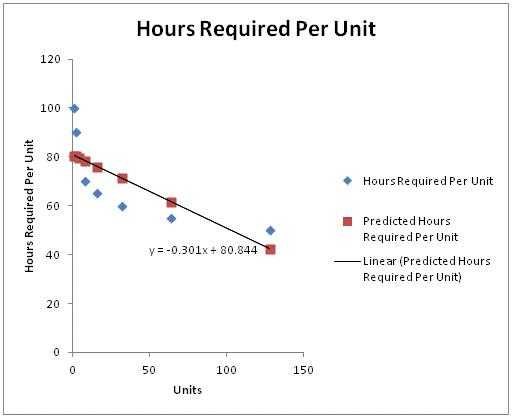
\includegraphics[scale=0.7]{assignment7-1.jpg}
\end{center}
\item Log-log scale graph of Hours Required Per Unit is provided below:
\begin{center}
	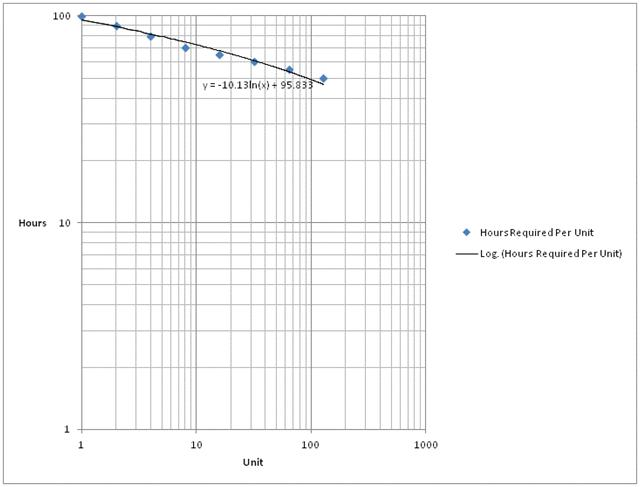
\includegraphics[scale=0.8]{assignment7-2.jpg}
\end{center}
\item The two graphs are significantly different.  The first graph shown the learning curve and does not follow very well with the predicted value liner relationship.  The log-log chart provides a much better linear representation to use for predicted values.
\item To find the predicted time for to manufacture the 150$^{\mbox{\scriptsize th}}$ unit, we utilized the Learning curve approach:
\begin{align*}
Y &= aX^{b} \\
A &= e^{\mbox{\scriptsize intercept}} \\
B &= \mbox{slope}
\end{align*}
We used the log values for the unit and hours and used regression in excel to find the $y$-intercept and slope as follows:
\begin{center}
	\begin{tabular}{l.}
	\hline
	\multicolumn{2}{c}{\textbf{Regression Statistics}} \\
	\hline\hline
	Multiple R & 0.996285293 \\
	R Square	& 0.992584385 \\
	Adjusted R Square	& 0.991348449 \\
	Standard Error	& 0.022464462 \\
	Observations	& 8 \\
	\hline
	\end{tabular}
	
	\begin{tabular}{lr....}
	\hline
	\myalign{c}{\textbf{ANOVA}} & \myalign{c}{\textbf{df}} & \myalign{c}{\textbf{SS}} & \myalign{c}{\textbf{MS}} & \myalign{c}{\textbf{F}} & \myalign{c}{\textbf{Significance F}} \\
	\hline\hline
	Regression	& 1	& 0.405	& 0.405	& 803.104 & 1.27792E-07 \\
	Residual	& 6	 & 0.003	& 0.001 & & \\
	Total	& 7	& 0.408 & & & \\
	\hline
	\end{tabular}
	
	\begin{tabular}{l....}
	\hline
	& \myalign{c}{\textbf{Coefficients}} &
	\myalign{c}{\textbf{Standard Error}} &
	\myalign{c}{\textbf{t Stat}} &
	\myalign{c}{\textbf{P-value}} \\
	\hline\hline
	Intercept & \cellcolor{yellow}4.584 & 0.015	& 316.140 & 6.76021E-14	\\ 
	Units	& \cellcolor{yellow}-0.142	& 0.005	& -28.339 & 1.27792E-07	\\
	\hline
	& \myalign{c}{\textbf{Lower 95\%}} &
	\myalign{c}{\textbf{Upper 95\%}} &
	\myalign{c}{\textbf{Lower 95.0\%}} &
	\myalign{c}{\textbf{Upper 95.0\%}} \\
	\hline
	Intercept & 4.549	 & 4.620 	& 4.549 	& 4.620 \\
	Units & -0.154	& -0.129	& -0.154	& -0.129 \\
	\hline
	\end{tabular}
\end{center}

For the 150$^{\mbox{\scriptsize th}}$ unit: 
\begin{align*} 
Y &= e^{4.58} \times 150^{-0.142} \\
&\approx 47.87
\end{align*}
The 150$^{\mbox{\scriptsize th}}$ unit would take approximately 48 hours
\item We use the same learning curve equation again for the 1000$^{\mbox{\scriptsize th}}$ unit:
\begin{align*}
Y &= e^{4.58}\times 1000^{-0.142} \\
&\approx 36.56
\end{align*}
The 1000$^{\mbox{\scriptsize th}}$ unit would take approximately 37 hours, this seems realistic as the learning curve is getting smaller and smaller.
\item Time to produce 150th unit = 48 hours. \\  Time to produce 300th unit = 37 hours.

Average time to produce between 150$^{\mbox{\scriptsize th}}$ and 300$^{\mbox{\scriptsize th}}$ unit $ = 48 +37/2 \approx 42.5 $. \\
Time to produce batch between 150$^{\mbox{\scriptsize th}}$h and 300$^{\mbox{\scriptsize th}}$ unit $= 42.5 * 150 \approx 6375 $ hours
\item 100 percent efficiency at 45 hours.  At the 150$^{\mbox{\scriptsize th}}$ unit we were at 48 hours.  The efficiency is calculated below:
\[ 45/48\times 100 = 94\% \mbox{\ efficiency} \]

After how many units do we reach optimal level:
\begin{align*}
45 &= e^{4.58}\times(\mbox{units})^{-0.142} \\
\frac{45}{97.5} &= (\mbox{units})^{-0.142} \\
0.46 &= (\mbox{units})^{-0.142} \\
237 &= \mbox{units is where you reach optimal level}
\end{align*}
\item After a six month break, assuming that we can assemble the same team for the first follow on contract, we expect them to be about 90\% efficient.  They would lose some of their efficiency just by the amount of time that lapses between production runs. \[ \frac{45}{0.9} = 50 \] We estimate 50 man hours/unit for the next 150 follow on contract with same team.
\item If the same team could not be assembled for the follow on contract, a greater reduction of efficiency would be expected.  However, it would not be greater than starting from scratch as many of the lessons learned have been documented.  Therefore, we expect an efficiency of 75\%. \[ \frac{45}{0.75} = 60 \] We estimate 60 man hours/unit for the next 150 follow on contract with different team.
\item At 60\% efficiency: \[ \frac{45}{0.6} = 75\mbox{\ hours} \] At 75\% efficiency:\[ \frac{45}{0.75} = 60\mbox{\ hours} \] $75 - 60 = 15$ hour reduction expected by the customer for each unit multiplied by 150 units equals a total of 2,250 hours at a cost of \$40/hr or a \$90,000 cost savings by increasing efficiency to 75\%.
\item The cost in training of new employees to get to required level of performance and the time it is going to take to get there must be considered when considering where to compromise in the efficiency factor.
\end{enumerate}

\section*{15-22}
A total of 3000 hours of direct labor is required for the effort.

\begin{enumerate}[a.]
\item How many direct labor hours per month per person (assume 8 hours per day and 40 hours per week):
\begin{itemize}
\item Vacation = 3 weeks $=3\times 40=120$ vacation hours per year \\
\item Sick days = 4 days  $=4\times 8=32$ sick hours per year \\
\item Paid holidays = 10 days $=10\times 8=80$  holiday hours per year \\
\item Jury duty = 1 day $=1\times 8=8$ jury duty hours per year \\
\item Total hours not worked per year $=120+32+80+8=240$ \\
\item Total hours available to work per year$=52 \mbox{\ weeks}\times 40 \mbox{\ hours per week}=2080$ \\
\item Total hours available per person per year $=2080-240=1840$ hours \\
\item Total direct labor hours per month per person $=1840/12=150.3$ hours
\end{itemize}
\item For one employee \[ 3000/153.3 =19.6 \] It would take one employee 19.6 months to complete the project.
\item \[ 3000/12 = 250 \] 250 hours must be completed each month for the project to be completed in 1 year. \[ 250/153.3 = 1.63 \] Therefore it will take two persons working on the project to complete in one year.
\end{enumerate}

\section*{15-24}
\begin{enumerate}[a.]
\item The cost and schedule variances are shown in the table below.
\begin{center}
  \begin{tabular}{c.....}
  	\hline
  	\myalign{c}{\textbf{Activity}} &
  	\myalign{c}{\textbf{BCWS}} &
  	\myalign{c}{\textbf{BCWP}} &
  	\myalign{c}{\textbf{ACWP}} &
  	\myalign{c}{\textbf{SV}} &
  	\myalign{c}{\textbf{CV}} \\
    \hline\hline
    	A & \$800.00 	 & \$1,000.00 	& \$1,100.00 & \$200.00 	& \$(100.00) \\
	B & \$1,200.00 &	 \$1,000.00 	& \$900.00  & \$(200.00)	& \$100.00 \\
	C & \$800.00 	 &	\$1,000.00 	& \$700.00 	& \$200.00 	& \$300.00 \\
	D & \$1,200.00 &	 \$1,000.00 	& \$1,100.00 	& \$(200.00)	& \$(100.00) \\
	E & \$1,000.00 &	 \$1,000.00 	& \$800.00 	& \$0.00   	& \$200.00 \\
    \hline
    & & & \myalign{c}{\textbf{Totals:}} & \$0.00 & \$400.00 \\
  \end{tabular}
\end{center}
\item Possible reasons for variances are listed for each of the activities below:
\begin{enumerate}[A]
\item \
\begin{itemize}
\item Accelerated schedule due to higher salaried personnel
\item Accelerated schedule due to overtime
\item Accelerated schedule due to additional resources
\end{itemize}
\item \
\begin{itemize}
\item Slippage due to lack of resources
\item Slippage due to mistakes
\item People are working but progress is poor
\item Over budget
\end{itemize}
\item \
\begin{itemize}
\item Accelerated schedule die to overlapping of activities
\item On schedule
\item On budget
\end{itemize}
\item \
\begin{itemize}
\item Slippage due to mistakes
\item People are working but progress is poor
\item Over budget
\end{itemize}
\item \
\begin{itemize}
\item On schedule
\item On budget
\end{itemize}
\end{enumerate}
\item The project appears to be \$400.00 over budget.
\item We would revise our answer above to reflect that the project appears to be \$400.00 under schedule and on budget.
\end{enumerate}

\section*{15-25}
\begin{enumerate}[a.]
\item The cost variances are shown in the table below.
\begin{center}
  \begin{tabular}{llr}
  	\hline
    	BCWS	& Dollars	 & \$29,750.00 \\
		& Hours	& 350 \\
	BCWP	& Dollars	 & \$34,000.00 \\
		& Hours	& 400 \\
	ACWP	& Dollars	 & \$38,400.00 \\
		& Hours	& 320 \\
	CV	& Dollars	 & \$(4,400.00) \\
		& Hours	& 80 \\
    \hline
  \end{tabular}
\end{center}
The cost variances confirm that we are both ahead of schedule and over budget.  Based solely on this information, it is reasonable to conclude that labor is highly effective albeit costly.  Given this situation, the project manager might request some less expensive resources from the line manager to integrate into the engineering process.  This would have the effect of slowing the schedule and also of slowing the burn rate of labor dollars.
\item The planned fully burdened labor rate using BCWS and BCWP both work out to \$85.00 per hour.
\item The actual fully burdened labor rate using ACWP works out to \$120.00 per hour.
\item The higher than anticipated labor rate can be narrowed down to a few factors including overtime hours worked, the use of senior (more expensive) labor, and unforeseen administrative/overhead costs.  Given the sizable increase in the actual labor rate, some adjustment will have to occur in order to hit a target budget.  Any adjustment that slows the schedule will only be effective if it also significantly reduces the labor costs in the process.  If the cost of internal labor is too great then outside (contractual) labor may be considered.  Even if the cost per hour is higher, the overhead is capped.  Given the information on hand, the project manager would be justified in asking the line manager for cheaper resources to integrate into the engineering and development process.
\item The calculated departmental overhead is 150\% for all pay grades except \emph{Apprentice Engineer}, whose overhead is 148\%.
\item This shows us that we can reduce labor costs only by using \emph{Apprentice Engineers} who may or may not be able to perform adequately.  The rate that was apparently budgeted was based on \emph{Junior Engineers} and labor dollars have been burned at a rate commensurate with \emph{Senior Engineers}.  One of the risks in changing the labor force mid-project is that any potential cost savings will be offset by an increased learning curve and reduced efficiency.  The project manager might look at the 13\% cost overrun in labor and see if it can be made up elsewhere in the project.  Other options include pitching a budget increase to senior leadership.  Given the significant reduction in schedule, a faster time to market might justify the labor overhead.
\end{enumerate}

\section*{Extra Question}
Risk Assessment:
\begin{itemize}
\item 80\% survival rate without smoking
\item 99.8\% survival rate with smoking with significantly increased chance of lung cancer
\end{itemize}

Since complete avoidance of risk is impossible and based on the information given and nothing else there are essentially two options for managing risk.  You can attempt control, avoid and mitigate the risk of tuberculosis infection without smoking.  This may be done through attempting to reduce your contact with infected people, wearing something to filter the air you breathe or possible medications to reduce infection rate.  The other option is to smoke and attempt to mitigate and control your risk of contracting lung cancer (thus controlling your risk of dying from tuberculosis).  Knowing that you dramatically increased your risk of lung cancer you can attempt to mitigate the severity of the lung cancer by being checked for it often so you can treat it in the earliest of stages if you do contract it.  You can also look into medications to control the risk of contraction.

Without anything additional information based of the effectiveness of the risk management techniques or to what degree smoking will increase your risk of lung cancer, we recommend smoking to decrease the risk of tuberculosis.  A 20\% mortality rate is a significant risk and reducing that to 0.2\% is very significant.  

\end{document}